\documentclass[sigconf, authorversion, nonacm]{acmart}
\settopmatter{printacmref=false}
\setcopyright{none}

\usepackage{booktabs}
\usepackage{graphicx}

\begin{document}

\title{Test-Guided, Scope-Aware Skill Evolution for Code Review Agents}
\subtitle{CSE 572 Data Mining, Group 22: Final Report}

\author{Pradnya Sanjeev Nidagundi}
\affiliation{\institution{Arizona State University}\city{Tempe}\state{AZ}\country{USA}}
\author{Sachin Venugopalan Nair}
\affiliation{\institution{Arizona State University}\city{Tempe}\state{AZ}\country{USA}}
\author{Aman Shrivastava}
\affiliation{\institution{Arizona State University}\city{Tempe}\state{AZ}\country{USA}}
\author{Sai Rithwik Kukunuri}
\affiliation{\institution{Arizona State University}\city{Tempe}\state{AZ}\country{USA}}

\renewcommand{\shortauthors}{Nidagundi, Nair, Shrivastava, and Kukunuri}

\begin{abstract}
Code review agents do not learn from their past reviews, even when test results later show which comments were useful. We study whether a review agent can improve by turning sanitized test feedback into short textual skills, and whether splitting those skills into global and pull request (PR) type tiers transfers better to unseen repositories than one global library under the same validation gate. We evaluate on c-CRAB, where a review counts as useful if a fixed repair agent acting on it makes a hidden test pass, with repository-disjoint splits and one open model (\texttt{qwen36-27b}) as reviewer, optimizer and repair agent. Before evolving anything we measured the noise the gate must clear: five identical runs on the same 34 selection PRs passed between 9 and 14 of 42 comments, and 8 PRs changed outcome. A gate calibrated to this noise needs a net gain of 5 PRs, so we ran evolution with the SkillOpt-style gate (net gain of 1) and report the calibrated gate as a sensitivity. Over six rounds the optimizer proposed six generic, correctness-focused global skills; the gate accepted one, with a net of +1, which is within the noise. On 70 held-out comments from 21 unseen repositories, the scoped library passed 12.9\% against 18.6\% for the global library (difference $-5.7$ points, 95\% CI $-15.5$ to $+4.3$, permutation $p = 0.44$). We find no detectable difference. At this benchmark size, repair noise and not skill organization decides most gate outcomes, and pass/fail feedback alone gives the optimizer too little to learn from.
\end{abstract}

\keywords{code review, LLM agents, skill evolution, repository shift, validation gating, evaluation noise}

\maketitle

\section{Introduction}
Code review catches defects and spreads knowledge within a team, but it takes a lot of developer time~\cite{bacchelli2013}. This has led to models that generate review comments~\cite{tufano2022pretrained, li2022codereviewer} and, more recently, to LLM agents that review whole PRs~\cite{zhang2026ccrab}. These agents are static. If a comment turns out to be useless, the agent will make the same kind of comment on the next PR.

LLM agents can improve without retraining by writing lessons into text that they read later~\cite{shinn2023reflexion, madaan2023selfrefine, zhao2024expel, wang2023voyager}. SkillOpt~\cite{yang2026skillopt} keeps such lessons in a skill library and accepts a change only if it helps on a validation set. Code review fits this idea well because c-CRAB~\cite{zhang2026ccrab} gives an objective signal: a comment is useful if acting on it makes a failing test pass.

Current skill methods keep one global list~\cite{yang2026skillopt, liu2026dynamics}. We think this is a problem for code review. Advice learned on bug fixes may not help on a new feature, and since only a few skills fit in the prompt, a wrong skill takes the place of a useful one. Our research question is: \textbf{under repository shift, does a library split into global and PR-type-scoped skills give a higher held-out c-CRAB pass rate than a single global library, when both use the same validation gate?} We expected the scoped library to pass more comments and to cause fewer regressions per accepted edit.

The comparison only means something if three conditions hold. No repository may appear in two partitions, so the test estimate measures transfer to unseen code. The two conditions must differ only in how the library is organized. And the test partition is scored once, after the system is frozen. We wrote these rules, the gate calibration and the analysis plan into a protocol before any final run~\cite{nosek2018prereg}, and we recorded every later change as a dated amendment.

The protocol also made us measure something our pilot could not: how much the outcome of the same review changes when the repair agent runs again. That measurement turned out to be the central result. Our contributions are:
\begin{enumerate}
\item a test-guided skill evolution pipeline for code review on c-CRAB, with repository-disjoint splits, a sanitized feedback channel that hides tests and gold comments from the optimizer, and a guarded, single-pass test partition;
\item a direct measurement of repair noise from five identical runs, and the gate threshold it implies;
\item a controlled comparison of scoped and global libraries under a shared gate, scored once on 70 held-out comments, which finds no detectable difference, with an analysis of what the optimizer actually proposed;
\item an account of why, at this sample size, the gate cannot separate real improvements from noise, and what a real test would need.
\end{enumerate}

\section{Related Work}
\textbf{Code review and its evaluation.} Bacchelli and Bird~\cite{bacchelli2013} found that developers mainly expect review to find defects, but much of it ends up being about code improvements and understanding. Pre-trained models such as those of Tufano et al.~\cite{tufano2022pretrained} and CodeReviewer~\cite{li2022codereviewer} generate review comments and score them by similarity to human comments, which rewards wording, not usefulness. SWE-bench~\cite{jimenez2024swebench} moved coding evaluation toward running real tests, and c-CRAB~\cite{zhang2026ccrab} brings this to code review: a fixed repair agent applies the review, and tests built from human review comments check whether the concern was fixed. The best of four released tools passes 32.1\% of comments, and all four together pass 41.5\%. Code Review Bench~\cite{zverianskii2026crb} instead scores precision and recall against human-verified findings.

\textbf{Self-improving agents.} Reflexion~\cite{shinn2023reflexion} and Self-Refine~\cite{madaan2023selfrefine} turn feedback into text that the next attempt reads. ExpeL~\cite{zhao2024expel} and Voyager~\cite{wang2023voyager} keep reusable insights or skills across tasks. OPRO~\cite{yang2024opro} and DSPy~\cite{khattab2024dspy} optimize prompts from scores. SkillOpt~\cite{yang2026skillopt} adds a validation gate to skill updates: a candidate is accepted if at least one more validation task passes and at most one regresses. Liu et al.~\cite{liu2026dynamics} show that gains can stall or reverse over many rounds.

\textbf{Noise in evaluation.} Benchmark scores of learned systems vary with seeds and run-to-run randomness, often by as much as the effects being compared~\cite{bouthillier2021variance}, and LLM code generation is non-deterministic even at temperature 0~\cite{ouyang2023nondeterminism}. Significance testing for paired system comparisons~\cite{dror2018hitchhiker} and the dangers of small, underpowered samples~\cite{button2013power} are well documented, as is leakage between training signal and evaluation~\cite{kapoor2023leakage}.

\textbf{Gap.} Skill-evolution methods use one global library, and c-CRAB has only evaluated static reviewers. We found no prior work that tests whether scoping skills by the type of change helps them transfer to new repositories, or that measures how noisy the validation signal is when the task outcome comes from a stochastic agent. SkillOpt's gate assumes a gain of one task is meaningful; Section~\ref{sec:calib} tests that assumption on c-CRAB.

\section{Data}
We use the public c-CRAB release~\cite{zhang2026ccrab}, pinned at commit \texttt{856dfa3}. Each instance is a Python PR with its diff, title, description, commits and one or more human review comments. Each comment has an executable test that fails before the fix and passes after it, so the outcome is pass or fail per comment. We reproduced the authors' filtering exactly (Table~\ref{tab:funnel}) and use the final 184 PRs (234 comments, 67 repositories). PR types come from the \texttt{problem\_domain} field: 67 bug fix, 68 feature and 49 other.

\begin{table}[t]
\caption{c-CRAB filtering, reproduced from the release.}
\label{tab:funnel}
\small
\begin{tabular}{lrr}
\toprule
Stage & PRs & Comments \\
\midrule
Full source test split & 671 & 1,313 \\
Comment filter (all have images) & 410 & 595 \\
Tests verified to fail, then pass & 339 & 485 \\
Resolved by repair agent (used) & 184 & 234 \\
\bottomrule
\end{tabular}
\end{table}

\textbf{Splits and eligibility.} Whole repositories are assigned to one partition with a fixed seed, using only repository size and PR type mix, never outcomes, and every partition contains all three PR types. Before any sampling we remove 8 PRs whose diffs exceed the reviewer's 120,000-character cap and 3 PRs with no accessible Docker image. Table~\ref{tab:splits} gives the eligible sets, which are the denominators for every number in this report. The released tools reach 35.7\% (Claude Code) and 44.3\% (all four) on the eligible test comments.

\begin{table}[t]
\caption{Repository-disjoint splits after eligibility filtering. BF / F / O: bug fix, feature and other PRs.}
\label{tab:splits}
\small
\setlength{\tabcolsep}{4pt}
\begin{tabular}{lrrrcl}
\toprule
Partition & PRs & Comm. & Repos & BF / F / O & Role \\
\midrule
Development & 87 & 107 & 25 & 34 / 31 / 22 & optimizer feedback \\
Selection & 34 & 42 & 17 & 14 / 6 / 14 & gate only \\
Test (locked) & 52 & 70 & 21 & 19 / 24 / 9 & scored once \\
\bottomrule
\end{tabular}
\end{table}

\textbf{Composition.} The selection set has only 6 feature PRs, while the test set has 24 of 52, so the gate sees little evidence about the PR type that dominates the test estimate. The \emph{other} tier aggregates seven source categories, so a skill learned for it draws on a mixture of change types.

\section{Methods}
\subsection{Pipeline}
For each PR, the reviewer gets the title, description and diff, plus up to 400 tokens of retrieved skills, and returns at most five findings as JSON. As in c-CRAB, Claude Code then applies the findings inside the PR's Docker image, and we run the PR's tests. A PR passes if all its tests pass, and a comment passes if its own test passes.

\textbf{Model.} All three roles use \texttt{qwen36-27b}, hosted by ASU, at temperature 0 with thinking disabled; a local LiteLLM proxy translates Claude Code's calls to that endpoint. Our progress-report pilot used Claude Sonnet 4.6 in all roles (4 of 16 development comments passed) at \$0.29 per PR evaluation, which made several thousand evaluations unaffordable. One model for every role keeps the internal comparison valid, but our absolute pass rates are not comparable to the released tools.

\textbf{Failures.} A repair timeout (1,200\,s), a Docker failure or an empty review is an infrastructure error. Errors count as failed in the primary metric and are excluded from gate counts, so an error is never a regression.

\subsection{Skills, optimizer and sanitizer}
A skill is a review instruction of at most 60 words, tagged global, bug fix, feature or other. In the \emph{global} condition all skills are global; in \emph{scoped}, retrieval adds the PR type's skills first and then global ones. Both use the same rules: a 400-token budget, newest first within a scope, duplicates removed, at most 6 skills per prompt. \emph{Static} retrieves nothing.

Each round evaluates the current library on all 87 development PRs and makes one optimizer call. The optimizer sees an allowlisted summary: pass counts per PR type, and up to 12 examples (failed PRs first) with the PR type, the reviewer's own findings with paths and line numbers removed, and how many of the PR's comments passed. It never sees diffs, test code, gold comments or selection results~\cite{kapoor2023leakage}; a check on the exact payload stops the run if any of these, a PR id or a repository name gets through. The optimizer proposes at most one edit per round (add, replace or delete) and is told which edits the gate already rejected.

\subsection{Validation gate and its calibration}
The current and candidate libraries are both evaluated on the 34 selection PRs. At the PR level, \emph{gained} counts PRs that fail with the current library and pass with the candidate, \emph{regressed} the reverse, and $\mathit{net} = \mathit{gained} - \mathit{regressed}$. A candidate is accepted if $\mathit{net} \geq \tau$ and $\mathit{regressed} \leq 1$.

SkillOpt fixes the threshold at one. Instead, before any evolution, we evaluated the unchanged (empty) library on the selection set five times with fresh draws: same prompts, PRs and seed, no cache. Any difference between these runs is noise. We set $\tau = \max(1, \lceil P_{95}(|\mathit{net}|)\rceil)$ over the nets of each repeat against the first.

Each gated condition runs at most 5 rounds and stops after 2 consecutive rejections; a rejected candidate leaves the library unchanged. Both conditions use the same PRs, seed and schedule. Results are cached by PR, retrieved skills and draw salt, so a library evaluated once is never re-drawn.

\subsection{Pre-registration and amendments}
The protocol was fixed on 2026-11-23, before any final-run data existed. The test partition is locked in code: unlocking requires a freeze record with the code hash, library hashes and test PR ids. Every later change is logged with its date and evidence, and none used test outcomes to choose anything.
\begin{itemize}
\item \textbf{A1}, before any evolution round: the calibrated threshold came out at $\tau=5$ (Section~\ref{sec:calib}), which would reject every edit and leave both libraries empty. We ran evolution at $\tau=1$, reported the calibrated gate's verdict for every round, and dropped the planned ungated ablation because $\tau=1$ is already close to ungated.
\item \textbf{A2--A4}, implementation bugs in Phase B: an off-by-one round count, empty-edit rounds not counting toward the stop rule, one firewall block on a single repair stopping a whole run, and two optimizer reply formats our parser dropped. We fixed each, logged the optimizer's raw replies from then on, and re-ran only the affected rounds.
\item \textbf{A5--A6}, the locked test: the first pass stopped at 37--38 of 52 PRs when a memory-heavy repair exhausted the shared 8\,GB host and the model proxy was killed. We capped each container at 1.5\,GB, made a persistent failure an error for that PR rather than a stop, re-froze with the new code hash (same libraries, test ids and salt), and resumed each pass once without re-drawing completed PRs. Partial pass counts had been printed to the run log; they did not inform any decision.
\item \textbf{A7}: an extension that gave the optimizer more detail about which kinds of concerns were missed was not run, because of time and compute limits (Section~\ref{sec:next}).
\end{itemize}

\subsection{Evaluation}
The primary metric is the comment-level pass rate on the locked test partition, errors counted as failed, over all 70 comments of the 52 eligible test PRs. The primary contrast is scoped versus global, two-sided. We report 95\% confidence intervals from a bootstrap that resamples the 21 test repositories (10,000 resamples)~\cite{efron1993bootstrap, field2007clustered}, because comments in one repository share conventions. The pre-registered test is a sign-flip permutation test on paired comment outcomes with whole repositories flipped (10,000 permutations); we also report McNemar's test~\cite{mcnemar1947} and its discordant counts~\cite{dror2018hitchhiker}. If a condition errors on more than 10\% of test PRs, we report the complete-case rate alongside.

\section{Results}
All numbers use \texttt{qwen36-27b} in every role. Sections~\ref{sec:static}--\ref{sec:evo} use no test data.

\subsection{Static baseline}\label{sec:static}
The static reviewer passes 26 of 107 development comments (24.3\%, 95\% CI 17.1--30.8\%) and 9 of 42 selection comments (21.4\%, CI 10.4--34.8\%). For reference, on the same eligible comments the released Claude Code passes 27.1\% and 42.9\%, and the union of all four tools 39.3\% and 47.6\%; these tools used their own models and repair setups, so this is not a controlled comparison.

\subsection{How noisy is the selection signal?}\label{sec:calib}
Table~\ref{tab:calib} shows five identical runs of the unchanged reviewer on the selection set. The pass rate ranged from 21.4\% to 33.3\%, a spread of 5 comments, with nothing changed but the random draw.

\begin{table}[t]
\caption{Five identical (A/A) runs on the selection set. Gained / regressed are PR-level against repeat 1, errored PRs excluded.}
\label{tab:calib}
\small
\begin{tabular}{lrrrc}
\toprule
Repeat & Passed / 42 & Rate & Errors & Gained / regr. / net \\
\midrule
1 & 9 & 21.4\% & 1 & --- \\
2 & 14 & 33.3\% & 1 & 5 / 0 / +5 \\
3 & 11 & 26.2\% & 0 & 2 / 0 / +2 \\
4 & 11 & 26.2\% & 2 & 2 / 0 / +2 \\
5 & 9 & 21.4\% & 0 & 4 / 2 / +2 \\
\bottomrule
\end{tabular}
\end{table}

\begin{figure*}[t]
\centering
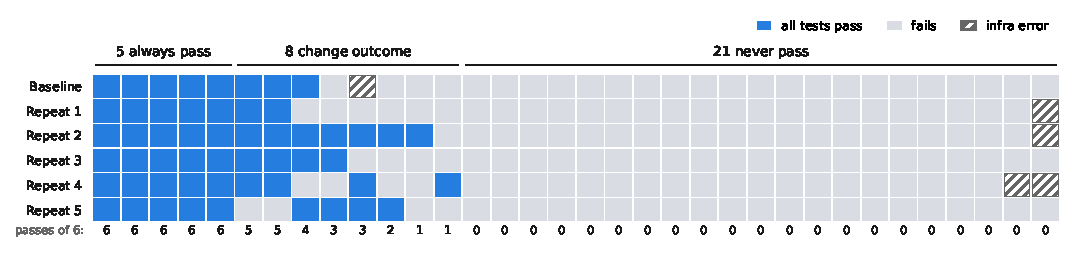
\includegraphics[width=\textwidth]{fig_calibration.pdf}
\caption{Outcome of each of the 34 selection PRs (columns) in the frozen baseline and five identical repeats (rows), sorted by how often the PR passes. Only 8 PRs ever change outcome; the other 26 pass always or never and carry no signal for a gate.}
\label{fig:calib}
\end{figure*}

\textbf{Threshold.} The 95th percentile of $|\mathit{net}|$ against repeat 1 is 4.55, so $\tau = 5$; all 10 pairs give the same $\tau$, with nets between $-3$ and $+5$.

\textbf{Where the noise comes from.} Figure~\ref{fig:calib} shows that the noise sits in a few PRs: 5 pass every time, 21 never pass, and 8 (23.5\%) change outcome. A candidate's net is mostly decided by which way those 8 fall in that run.

\textbf{What a gate accepts by chance.} Applied to ordered pairs of identical runs, the $\tau = 1$ rule accepted 6 of 20 (30\%), and the SkillOpt rule ($\mathit{gained} \geq 1$, $\mathit{regressed} \leq 1$) also 6 of 20. A null edit passes a SkillOpt-style gate about a third of the time. At $\tau = 5$, a real edit would have to beat the largest difference we saw between two identical runs.

\subsection{Evolution}\label{sec:evo}
Table~\ref{tab:evo} and Figure~\ref{fig:gate} show every evaluated round. Global stopped after two rejections; scoped accepted one edit in round 2 and then stopped after two more rejections.

\begin{table*}[t]
\caption{Every evaluated evolution round. Selection: comments passed out of 42, current library $\rightarrow$ candidate. G / R: selection PRs gained / regressed. $\tau=1$ is the operating gate (A1); $\tau=5$ the calibrated one. All proposals are global-scope adds.}
\label{tab:evo}
\small
\setlength{\tabcolsep}{4pt}
\begin{tabular}{llp{7.6cm}rcrrcc}
\toprule
Condition & Round & Proposed skill (opening words) & Words & Selection & G / R & Net & $\tau=1$ & $\tau=5$ \\
\midrule
Global & 1 & ``Prioritize identifying runtime errors \ldots\ over stylistic or documentation issues'' & 46 & 10 $\rightarrow$ 5 & 1 / 5 & $-4$ & reject & reject \\
Global & 2 & ``Verify type consistency in set operations \ldots\ convert dict\_keys to set'' & 56 & 10 $\rightarrow$ 8 & 1 / 4 & $-3$ & reject & reject \\
Scoped & 1 & ``Prioritize high-impact correctness issues \ldots\ avoid nitpicking documentation or style'' & 30 & 10 $\rightarrow$ 8 & 0 / 3 & $-3$ & reject & reject \\
Scoped & 2 & ``Validate API contract compliance: arguments match expected types, keys exist \ldots'' & 49 & 10 $\rightarrow$ 11 & 2 / 1 & $+1$ & \textbf{accept} & reject \\
Scoped & 3 & ``Verify semantic correctness of logic, not just syntax \ldots'' & 42 & 11 $\rightarrow$ 13 & 1 / 1 & $0$ & reject & reject \\
Scoped & 4 & ``Verify variable scope and initialization order to prevent UnboundLocalError \ldots'' & 55 & 11 $\rightarrow$ 10 & 0 / 2 & $-2$ & reject & reject \\
\bottomrule
\end{tabular}
\end{table*}

\begin{figure}[t]
\centering
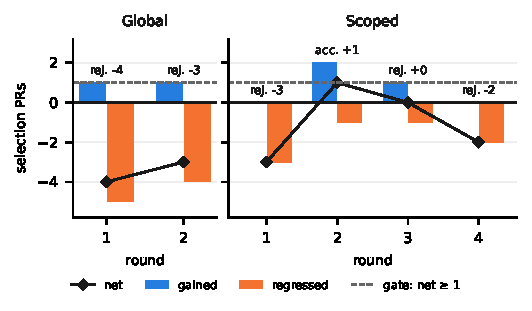
\includegraphics[width=\columnwidth]{fig_gate.pdf}
\caption{Selection PRs gained (up) and regressed (down) per round, with the net. The dashed line is the operating gate's net threshold.}
\label{fig:gate}
\end{figure}

\textbf{One edit was accepted, and it is indistinguishable from noise.} Five of six candidates had a net of 0 or below, and global round 1 regressed 5 PRs. The one acceptance had a net of +1; identical runs produced +1 and +2, and the calibrated gate would have rejected every candidate. The frozen libraries are therefore \emph{global}: empty, and \emph{scoped}: one global skill.

\textbf{The accepted skill did not help on development either.} With it, the development pass passed 21 of 107 comments (19.6\%, 2 errors) against 26 of 107 for the static reviewer.

\textbf{The optimizer never used scoping.} All six proposals are global, including the four in the scoped condition, which could have written type-specific skills. Each tells the reviewer to look harder for correctness problems (undefined variables, types, imports, API contracts), and two tell it to avoid style and documentation comments. The specific details (dict\_keys, error codes, HTTP status codes) come straight from the reviewer's own findings on PRs where the review failed. The optimizer sees \emph{that} those reviews failed, not \emph{what} the human reviewer asked for, so it can only restate the failed review in more general words.

\subsection{Locked test}\label{sec:test}
Each frozen library was scored once on the 52 test PRs with the same test salt (Table~\ref{tab:test}, Figure~\ref{fig:test}).

\begin{table}[t]
\caption{Locked test pass: comment-level pass rate, errors counted as failed, with repository-clustered 95\% CIs. CC: complete-case rate, which excludes the comments of errored PRs.}
\label{tab:test}
\small
\setlength{\tabcolsep}{3.5pt}
\begin{tabular}{lrcrrr}
\toprule
Condition & Passed & Rate [95\% CI] & PRs & Err. & CC \\
\midrule
Static & 13 / 70 & 18.6\% [10.8, 27.8] & 9 / 52 & 5 & 21.0\% \\
Global & 13 / 70 & 18.6\% [10.8, 27.8] & 9 / 52 & 5 & 21.0\% \\
Scoped & 9 / 70 & 12.9\% [5.3, 21.6] & 7 / 52 & 6 & 14.1\% \\
\bottomrule
\end{tabular}
\end{table}

\begin{figure}[t]
\centering
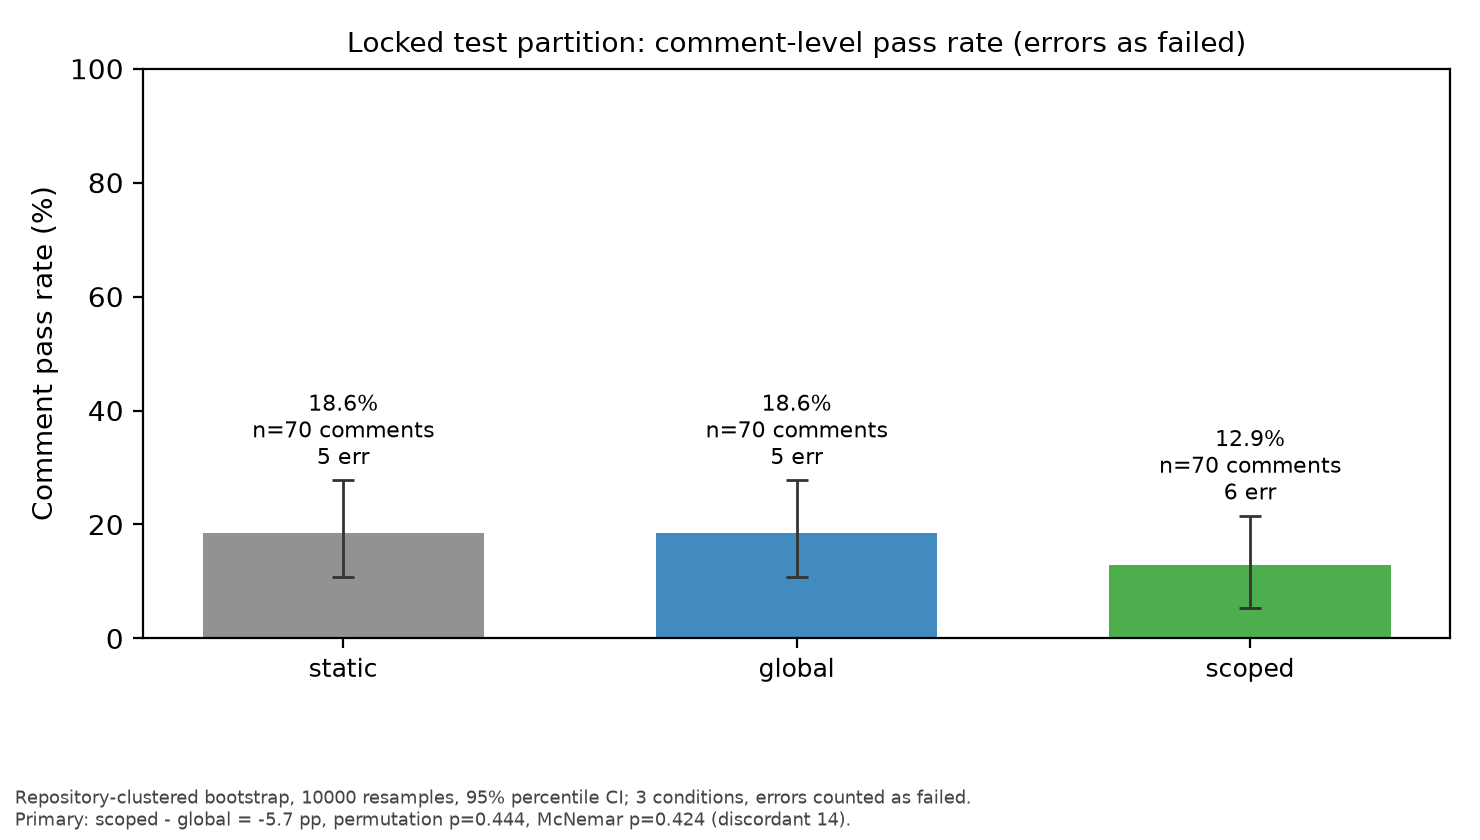
\includegraphics[width=\columnwidth]{fig_test_comparison.png}
\caption{Comment-level pass rate on the locked test partition with repository-clustered 95\% intervals.}
\label{fig:test}
\end{figure}

\textbf{Primary contrast.} Scoped minus global is $-5.7$ points (95\% CI $-15.5$ to $+4.3$; permutation $p = 0.44$). Of the 70 paired comments, 14 are discordant: 5 pass only under scoped and 9 only under global (exact McNemar $p = 0.42$). At the PR level scoped gained 3 PRs and lost 5. There is no detectable difference, and the point estimate is in the opposite direction from our hypothesis.

\textbf{Global equals static.} Both froze an empty library and share a test salt, so they share every cached draw; they agree on all 70 comments, errors included.

\textbf{Errors, PR types and transfer.} Scoped errored on 6 of 52 PRs (11.5\%), above our 10\% bar; its complete-case rate (14.1\% against 21.0\%) gives the same ordering. Scoped passes fewer feature comments than global (2 against 6 of 37) and fewer bug-fix comments (6 against 7 of 23), counts too small to read further. Selection overstated test performance for every condition: by 2.9 points for static and by 13.3 points for scoped, whose selection estimate (26.2\%) comes from the very run that accepted its skill.

\textbf{Cost.} Hosting was free, so we count tokens and time. More than 99\% of tokens are the repair agent's prompts. On the test pass, static used 3.0M tokens and 39 minutes of review-plus-repair time per PR that passed all its tests; scoped used 4.7M tokens and 44 minutes, spending more per PR (636k against 522k tokens) and passing fewer. Runs moved from a laptop, where the amd64 images ran under emulation, to a 4-core x86 server, where a repair took 91\,s instead of about 230\,s; memory, not CPU, then limited parallelism.

\section{Discussion}
\subsection{The gate cannot see effects this small}
Two identical runs differed by up to 5 of 34 PRs, and 8 PRs changed outcome with nothing changed. Any gate on this signal is either too strict to accept anything ($\tau=5$) or loose enough to accept about a third of null edits ($\tau=1$ and the SkillOpt rule). This is a property of the measurement, not of the scoped design or our optimizer: it holds for any method that validates skill edits on a few dozen c-CRAB PRs with a stochastic repair agent~\cite{bouthillier2021variance, ouyang2023nondeterminism}, and it applies to the SkillOpt gate as published, which treats one extra passing task as evidence. With 52 test PRs, the test comparison is also underpowered for effects of a few points~\cite{button2013power}.

\subsection{What our comparison tests}
Under A1 both libraries evolved under a permissive gate, so accepted edits were not filtered for quality. The test result fits that reading. The one edit the gate let through was a generic, global skill accepted on noise; it came out 5 comments worse on development and 4 worse on test, so the scoped library ended up below the empty one. Because scoped never wrote a PR-type skill, the result says nothing for or against scoping itself. It is evidence that a permissive gate on a noisy signal lets weak edits through, and that the optimizer, given pass/fail feedback, had nothing better to offer.

\subsection{What a real test would need}\label{sec:next}
\textbf{A richer signal.} The feedback says that a review failed but not why. A natural next step is to tell the optimizer what \emph{kind} of concern was missed, without the gold wording, file or line: for example, a coarse category per missed comment and whether any finding touched the right file. That would also give it a reason to write PR-type skills. Time and compute limits prevented us from exploring this, and it is the first thing we would study next.

\textbf{A quieter measurement.} A gate can only detect an effect larger than its noise. Three changes would help: evaluate each candidate several times and gate on the mean; drop the PRs that always or never pass, which carry no information, and spend the budget on the unstable ones; and use a larger selection set, since the noise in \emph{net} grows roughly with the square root of the set size while a real per-PR effect grows linearly.

\subsection{Limitations}
A 27B open model plays every role, so absolute pass rates are not comparable to the released tools or to our Sonnet pilot. Compute limited how many repeats we could afford. We did not run a control that replaces the reviewer's findings with generic text, so we cannot say how much of the repair agent's success comes from the findings rather than the diff. Four test PRs have JavaScript tests and may fail for environment reasons. We dropped Code Review Bench as an outside test set and did not run the planned blind labelling of findings. The selection set has only 6 feature PRs. Completed test PRs ran before the memory cap of A6 and the remaining ones after it.

\section{Conclusion}
We built a test-guided skill evolution pipeline for code review agents, with repository-disjoint splits, a feedback channel that hides tests and gold comments from the optimizer, and a test partition scored once. Before evolving anything, we measured that the selection outcome changes by up to 5 of 34 PRs between identical runs. A gate calibrated to that noise accepts nothing, and a SkillOpt-style gate accepts about a third of edits that change nothing. On 70 held-out comments the scoped library, holding one accepted skill, passed 12.9\% against 18.6\% for the empty global library, a difference we cannot distinguish from zero, and the optimizer never used the scoping it was offered. Whether scoped skills transfer better than global ones remains open. Testing it on c-CRAB needs feedback that says what a review missed and a validation signal several times less noisy than one run per PR.

\bibliographystyle{ACM-Reference-Format}
\bibliography{references}

\end{document}
